%
\hsection{Adding Rows to a Table and Executing Views}%
\label{sec:factory:tableAndView}%
\FloatBarrier%
%
\begin{figure}%
\centering%
%
\subfloat[][%
We double-click on the table~\sqlil{demand} in the \inQuotes{Tables} pane.%
\label{fig:factoryLibreOfficeBaseTableAndView1chooseTableDemand}%
]{\tightbox{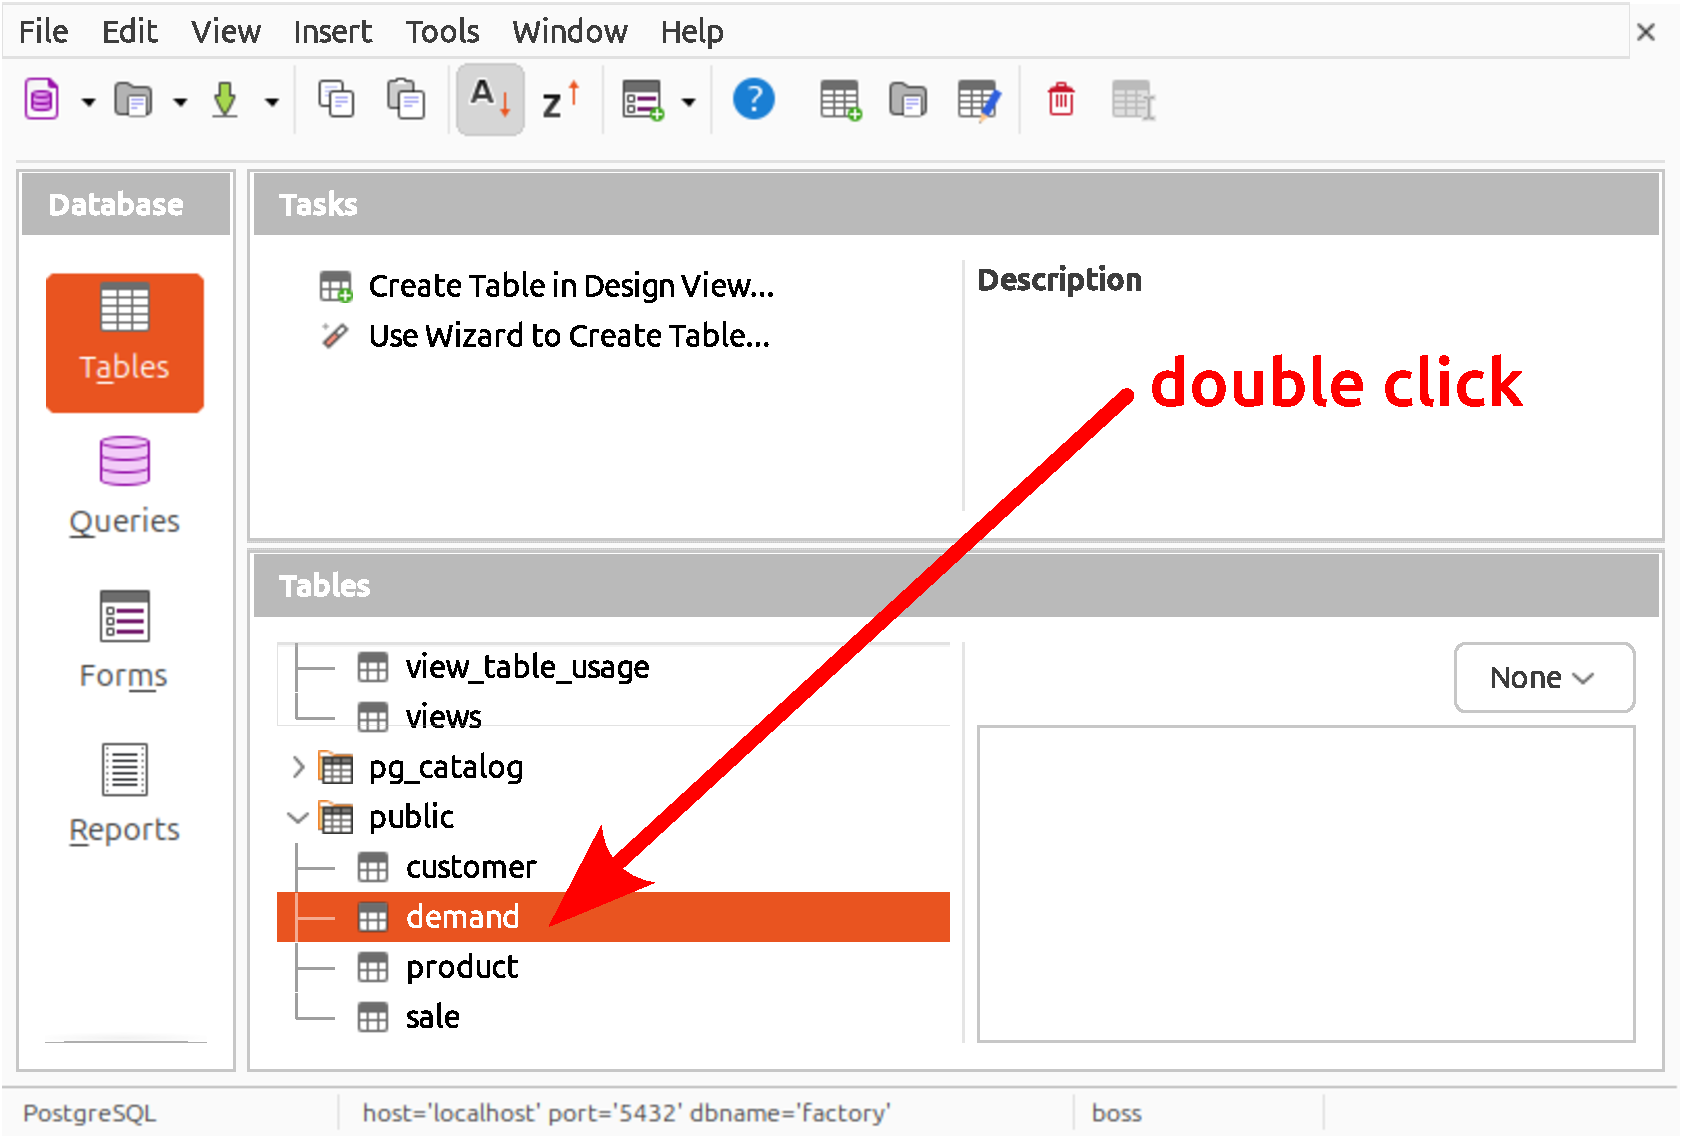
\includegraphics[width=0.49\linewidth]{\currentDir/factoryLibreOfficeBaseTableAndView1chooseTableDemand}}}%
%
\floatSep%
%
\subfloat[][%
The table \sqlil{demand} opens in a separate window, displaying the table content. %
Click into the second cell in the empty row at the bottom.%
\label{fig:factoryLibreOfficeBaseTableAndView2tableDemand}%
]{\tightbox{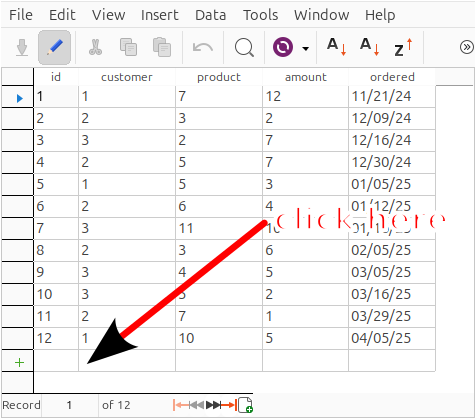
\includegraphics[width=0.49\linewidth]{\currentDir/factoryLibreOfficeBaseTableAndView2tableDemand}}}%
%
\floatRowSep%
%
\subfloat[][%
We enter a new row of data, leaving the \sqlil{id} column empty. %
When reaching the end of row, i.e., after entering all the data, we press~\keys{\tab}.%
\label{fig:factoryLibreOfficeBaseTableAndView3addDemand}%
]{\tightbox{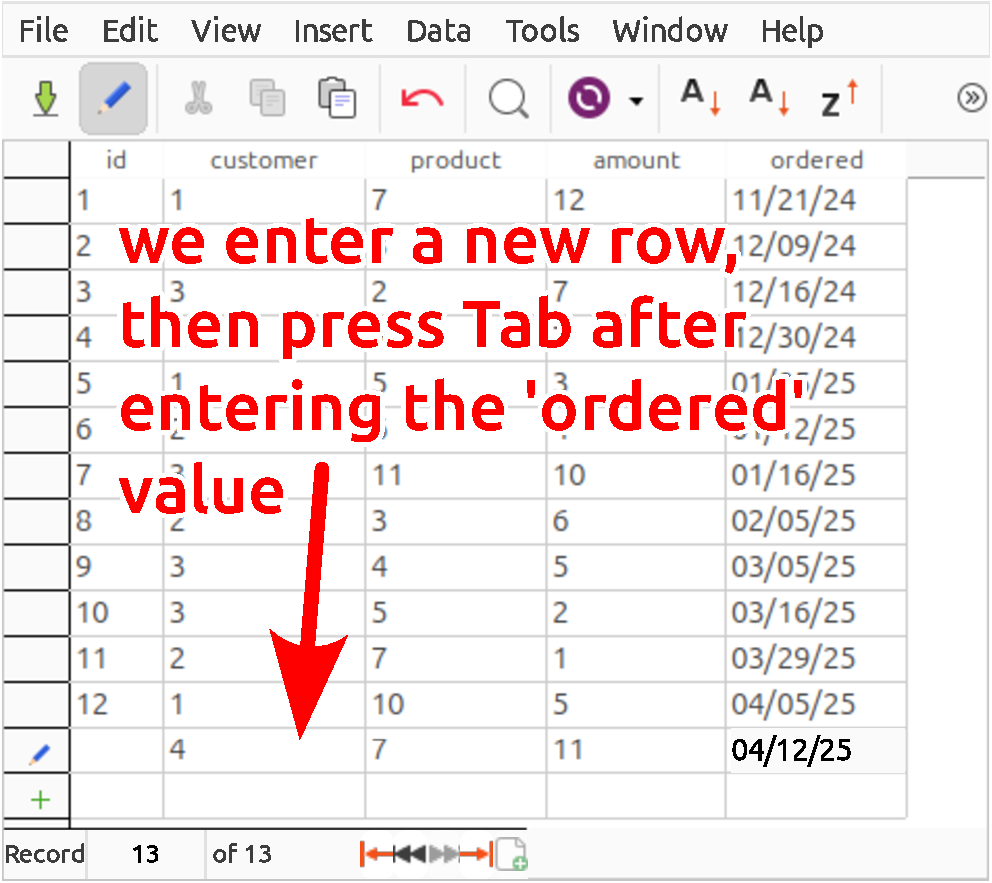
\includegraphics[width=0.49\linewidth]{\currentDir/factoryLibreOfficeBaseTableAndView3addDemand}}}%
%
\floatSep%
%
\subfloat[][%
The row has now been sent to the \dbms. %
It has not been loaded back from the \dbms, so the \sqlil{id} is still~0. %
We click on the \inQuotes{reload} option.%
\label{fig:factoryLibreOfficeBaseTableAndView4demandAdded}%
]{\tightbox{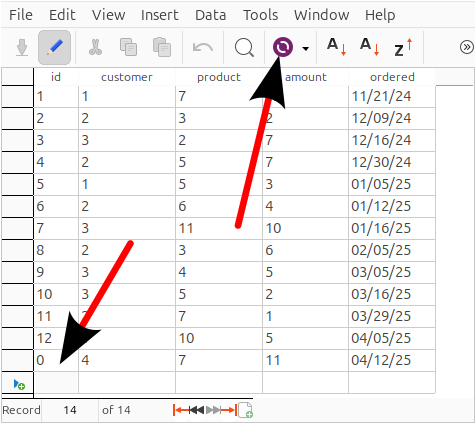
\includegraphics[width=0.49\linewidth]{\currentDir/factoryLibreOfficeBaseTableAndView4demandAdded}}}%
%
\caption{Adding a row to the table \sqlil{demand} and executing the view \sqlil{sale} from \libreofficeBase.}%
\label{fig:factoryLibreOfficeBaseTableAndViewA}%
%
\end{figure}%
%
\begin{figure}%
\ContinuedFloat%
\centering%
%
\subfloat[][%
After refreshing the data by pressing~\libreOfficeBaseRefresh, the \sqlil{id} field is now~13 as it should be.%
\label{fig:factoryLibreOfficeBaseTableAndView5demandsRefreshed}%
]{\tightbox{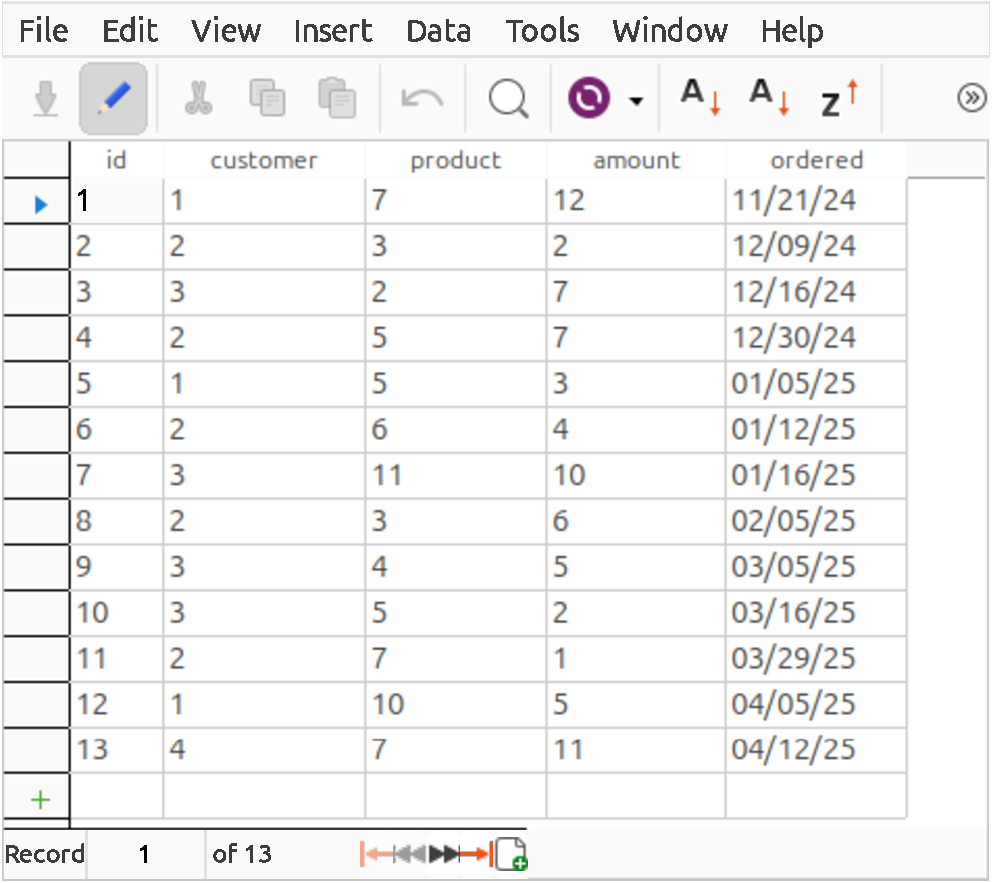
\includegraphics[width=0.49\linewidth]{\currentDir/factoryLibreOfficeBaseTableAndView5demandsRefreshed}}}%
%
\floatRowSep%
%
\subfloat[][%
We now double-click on the view~\sqlil{sale} in the \inQuotes{Tables} pane.%
\label{fig:factoryLibreOfficeBaseTableAndView6chooseViewSale}%
]{\tightbox{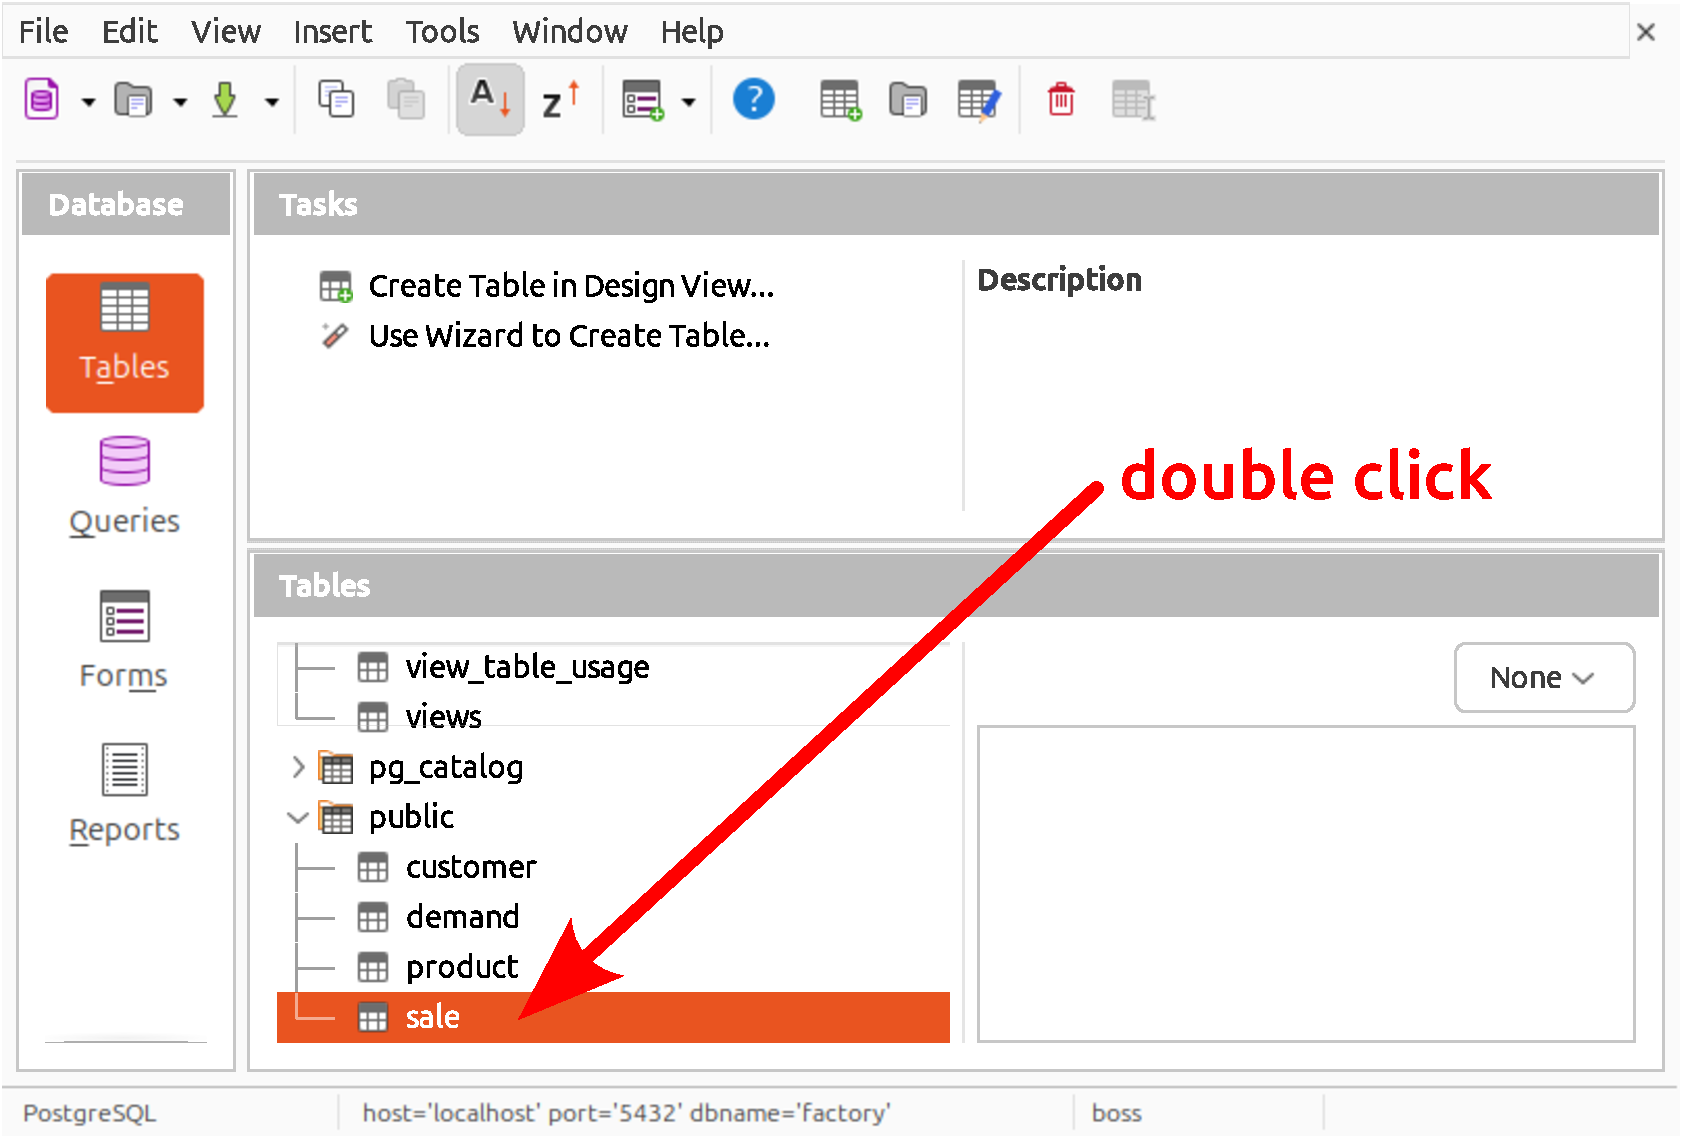
\includegraphics[width=0.49\linewidth]{\currentDir/factoryLibreOfficeBaseTableAndView6chooseViewSale}}}%
%
\floatSep%
%
\subfloat[][%
The view is executed as expected. %
The newly entered demand also showed up: %
There now is a sale for Mr.~Bobbo.%
\label{fig:factoryLibreOfficeBaseTableAndView7viewSale}%
]{\tightbox{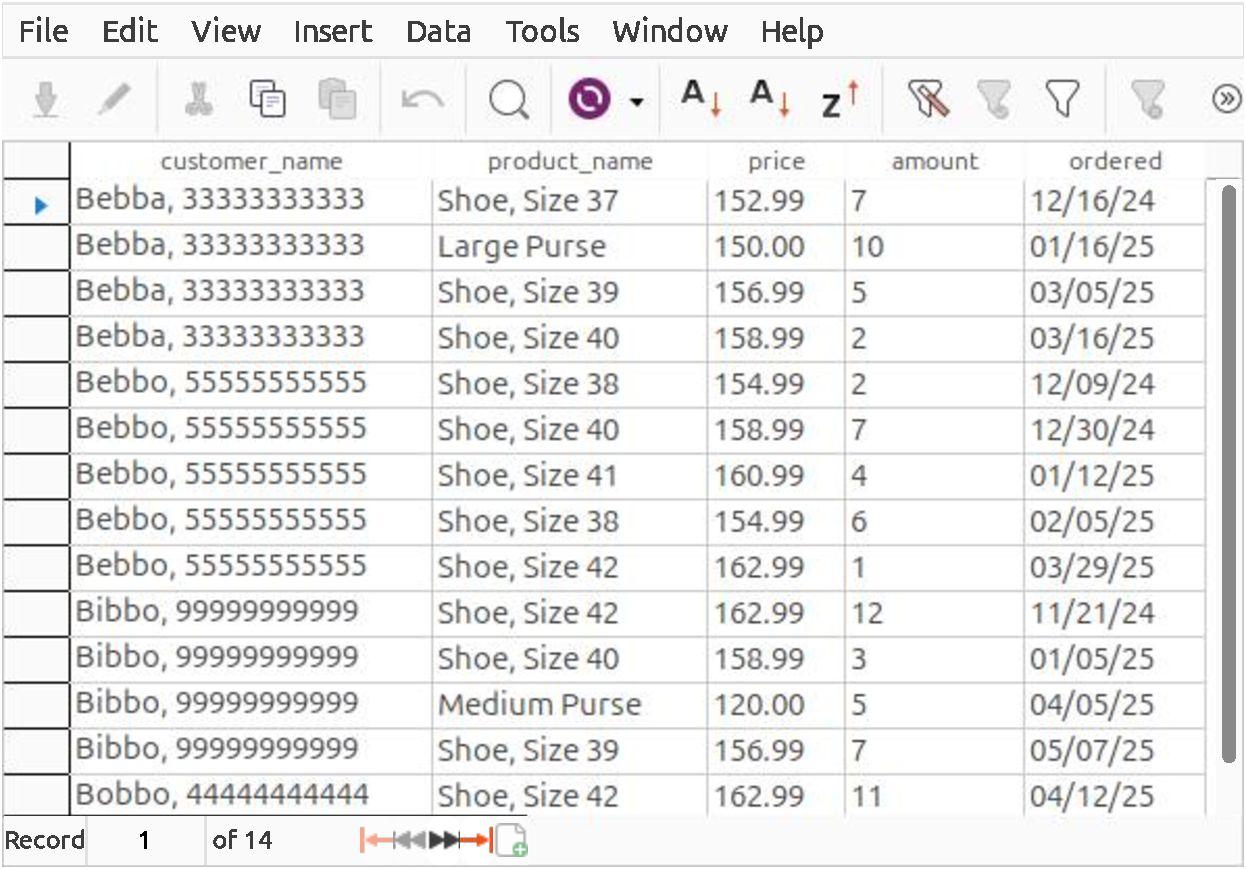
\includegraphics[width=0.49\linewidth]{\currentDir/factoryLibreOfficeBaseTableAndView7viewSale}}}%
%
\caption{Adding a row to the table \sqlil{demand} and executing the view \sqlil{sale} from \libreofficeBase.}%
\label{fig:factoryLibreOfficeBaseTableAndViewB}%
\end{figure}%
%
We now can use \libreofficeBase\ as a simple \pgls{GUI} to enter data into our \db.
For trying this, we select the table \sqlil{demand} in the \inQuotes{Tables}~pane and double-click on it in \cref{fig:factoryLibreOfficeBaseTableAndView1chooseTableDemand}.
A new window opens.
In this window, we see the contents of the table.
We can edit them there.
For example, we can place the cursor into the second field of the empty row at the bottom~\cref{fig:factoryLibreOfficeBaseTableAndView2tableDemand}.
(We skip the \sqlil{id} column, because its value can automatically be set by the \dbms.)
As data, we choose customer id~4, which refers to Mr.~Bobbo in~\cref{fig:factoryLibreOfficeBaseTableAndView3addDemand}.
One April~12, 2025, he ordered 11 units of the product with id~7, i.e., shoes of size~37.

After entering this data, when our cursor is in the last cell of the row, we press~\keys{\tab}.
The new record is sent to the \dbms\ in~\cref{fig:factoryLibreOfficeBaseTableAndView4demandAdded}.
Notice that, at this stage, the window displays the \sqlil{id} field of the new row as~0.
The reason is that we did not enter any value here.
The system has sent the new row to the \dbms.
The \dbms\ then sets the \sqlil{id} field automatically.
However, the \libreofficeBase\ \pgls{GUI} does not know this.
In order to see the actual value of the field~\sqlil{id}, we have to reload the data.

We therefore click on the refresh button~\libreOfficeBaseRefresh\ in \cref{fig:factoryLibreOfficeBaseTableAndView5demandsRefreshed}.
Indeed, now the \sqlil{id} field has the new and correct value~13.
We close the table window and go back to the main window.

Back to the \inQuotes{Tables} pane we now double-click on the view \sqlil{sale} in \cref{fig:factoryLibreOfficeBaseTableAndView6chooseViewSale}.
This again opens a new window in \cref{fig:factoryLibreOfficeBaseTableAndView7viewSale}.
We now see the results of the query in a nice tabular form.
It may be that the \sqlil{customer_name} column is displayed a bit odd on your computer.
In this case, just resize it and make it a bit wider by dragging its right border to the left with the mouse.
Then all the data will appear correctly.

Remember that above, we just added a new demand into our table?
Back in \cref{exec:factory:select_from_view_sale_3}, there was not a single order for Mr.~Bobbo in our system.
But now one appears in the view window, at the bottom row.
In other words, the view has been executed and led to the expected results, also proving that our changes to the \db\ were indeed persistently stored.%
%
\FloatBarrier%
\endhsection%
%
